
\chapter{绪论}
\section{研究背景及意义}
\subsection{分布式训练的发展}

% 过去十余年，深度学习在计算机视觉、自然语言处理与科学计算等方向持续取得突破，其核心推动力来自于模型结构创新与算力基础设施的共同演进。\cite{fukushima1980neocognitron,he2016deep,vaswani2017attention} 伴随数据体量与任务复杂度的提升，训练过程逐渐从“单机可完成”走向“必须依赖集群协同”。一方面，典型视觉数据集（如 ImageNet）规模已达到百 GB 量级\cite{deng2009imagenet}；另一方面，大模型参数量快速攀升，包含大量稀疏或密集的矩阵运算，使得训练所需计算量呈指数式增长\cite{fedus2022switch,zhang2022opt,brown2020language}。近年来大规模神经网络模型的参数规模变化如\autoref{fig:Fig1-1}所示。

% \captionsetup[figure]{labelformat=simple, labelsep=space}
% \begin{figure}[!htbp]
%     \centering
%     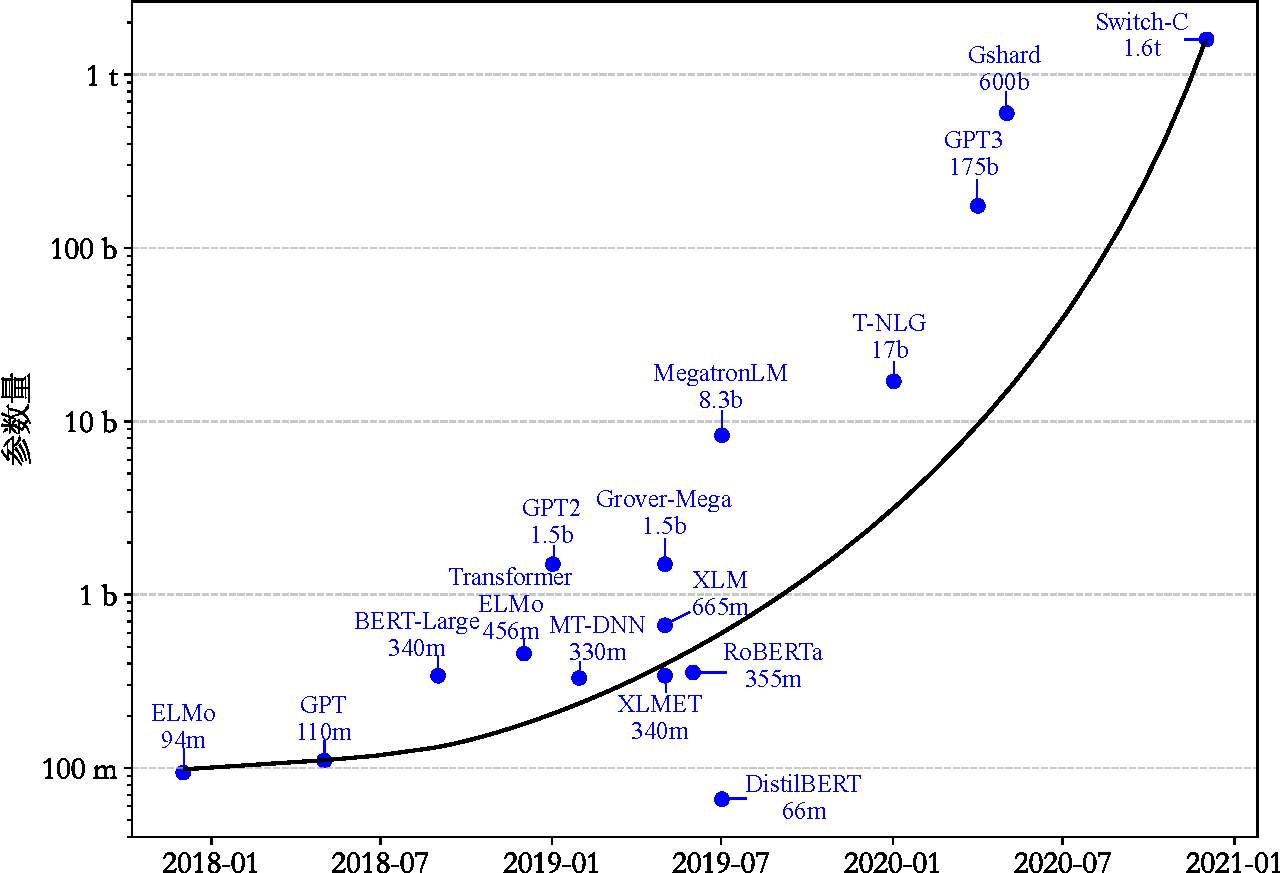
\includegraphics[width=5in]{figure/chapter1/fig1-1-nn_params.pdf}
%     \caption{\label{fig:Fig1-1}大规模深度神经网络模型的发展情况（数据来源：OpenAI）}
% \end{figure}

% 与模型和数据的增长相比，单卡算力提升速度相对有限。以 NVIDIA GPU 为例，\autoref{tab:GPU性能} 给出了不同代际 GPU 在训练 ResNet 模型时的性能表现\cite{luo2018parameter}。可以看到，硬件吞吐的提升并不足以抵消训练规模扩张带来的压力；同时，超大模型对显存容量与带宽提出更高要求，单设备往往难以容纳完整模型或满足端到端吞吐需求。由此，采用多 GPU/NPU 的分布式训练成为业界主流路径\cite{ben2019demystifying}。

% \begin{table}[!htbp]
%     \centering
%     \caption{单GPU训练ResNet-269模型的性能\cite{luo2018parameter}}
%     \label{tab:GPU性能}
%     \setlength{\tabcolsep}{5mm}{
%             \begin{tabular}{ccc}
%                 \toprule[2pt]
%             \multicolumn{1}{l}{GPU型号} & \multicolumn{1}{l}{发布时间} & \multicolumn{1}{l}{训练速度（图片/秒）} \\ \midrule[1pt]
%             K520                     & 2012年 &4     \\
%             K80                  & 2014年 &11        \\
%             M60                     &2015年 & 14  \\
%             1080Ti                   & 2017年 & 44\\ 
%             V100                   &2019年& 65     \\\bottomrule[2pt]

%             \end{tabular}
%     }
% \end{table}

% 从优化角度看，分布式训练将总体目标拆分为多个节点上的局部计算，并通过通信保持不同节点之间的一致性。对由 $n$ 个节点构成的训练任务，常用形式可写为\cite{smola2010architecture}：
% \begin{equation}
%     \label{equ:distributed_training_optimization_object}
%     \min_x \!\:F\left( x \right) \coloneqq \frac{1}{n}\sum_{i=1}^n{\underset{=:f_i(x)}{\underbrace{\mathbb{E}_{\xi _i\sim D_i}l(x;\xi _i)}}}
% \end{equation}
% 其中 $x\in \mathbb{R}^d$ 为模型参数，$D_i$ 为节点 $i$ 的本地数据分片，$l(\cdot)$ 表示样本损失函数。实际训练中，如何在保证数值语义与模型精度的前提下高效完成“计算—通信—同步”闭环，是决定训练效率的关键。

% 现有分布式训练通常同时涉及多种并行方式。\cite{tang2020communication} 如\autoref{fig:Fig1-2} 所示，数据并行（Data Parallelism）将数据分片到不同设备上，每个设备持有完整模型副本，迭代过程中需要频繁同步梯度/参数；模型并行（Model Parallelism）则将模型结构或张量维度切分到多设备上，通过中间激活值与梯度的交换完成前向与反向计算。在大模型训练中，模型并行往往进一步细分为张量并行、流水并行与专家并行等形式，它们在不同层级引入 AllReduce、ReduceScatter、AllGather、AlltoAll 以及点到点通信等操作，通信模式更为密集且更接近关键路径。

% \begin{figure}[!htbp]
%     \centering
%     \subfigure[数据并行训练方式]{
%         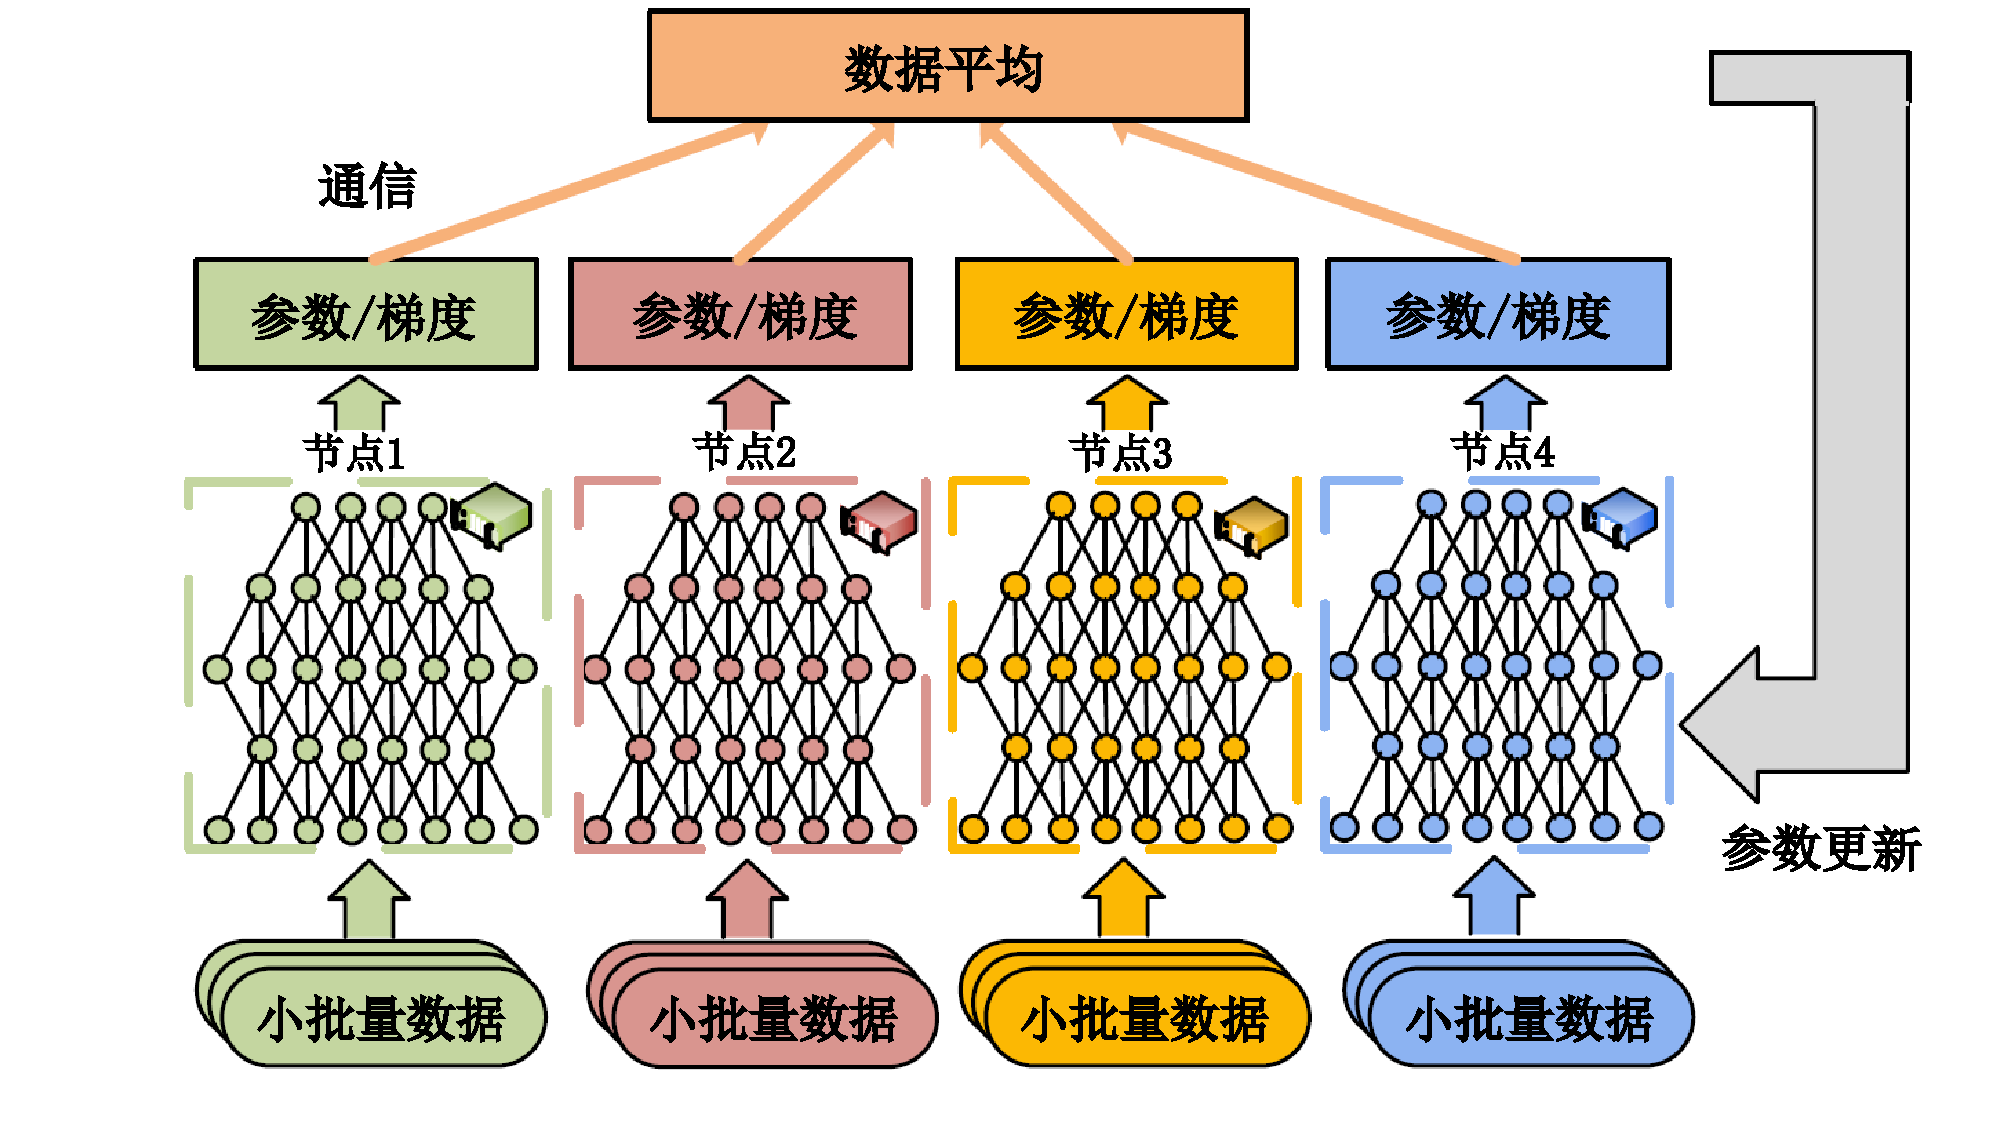
\includegraphics[width=0.5\linewidth]{figure/chapter1/fig1-2-data_parallel.pdf}
%         \label{fig:Fig1-2-data-parallel}
%     }
%     \subfigure[模型并行训练方式]{
%         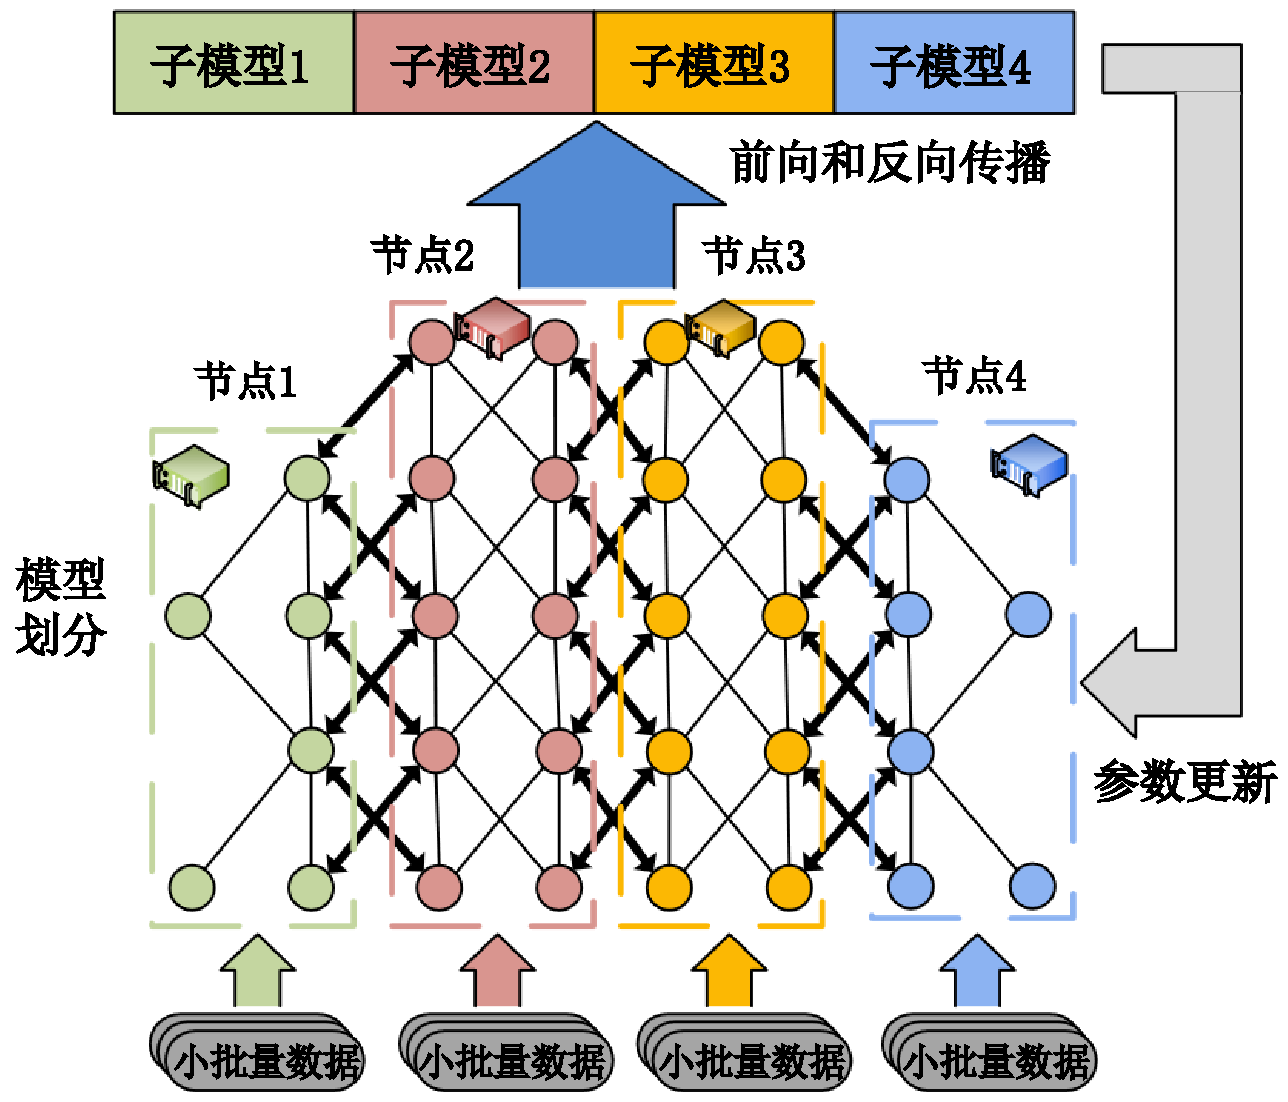
\includegraphics[width=0.4\linewidth]{figure/chapter1/fig1-2-model_parallel.pdf}
%         \label{fig:Fig1-2-model-parallel}
%     }
%     \caption{分布式深度学习并行训练方式}
%     \label{fig:Fig1-2}
% \end{figure}

% 在系统实现层面，分布式训练的通信组织方式主要包括参数服务器（PS）架构\cite{li2014communication}、基于集合通信的 All-Reduce 架构\cite{sergeev2018horovod}，以及去中心化的 Gossip 架构\cite{kempe2003gossip,lian2017can}。其中，PS 架构易于理解但中心节点可能成为瓶颈；Gossip 架构通信灵活、容错性好，但一致性收敛与调度设计更复杂。相比之下，All-Reduce 及其相关集合通信算子（AllReduce/ReduceScatter/AllGather/AlltoAll）能够直接服务于数据并行、张量并行与专家并行等训练方式，且更容易与高性能互连硬件及主流通信库（如 NCCL、HCCL 等）对接，因此在当前大规模训练系统中应用最为广泛。本文的研究工作也将围绕集合通信算子及其与计算过程的协同优化展开。

% \begin{figure}[!htbp]
%     \centering
%     \subfigure[PS架构]{
%         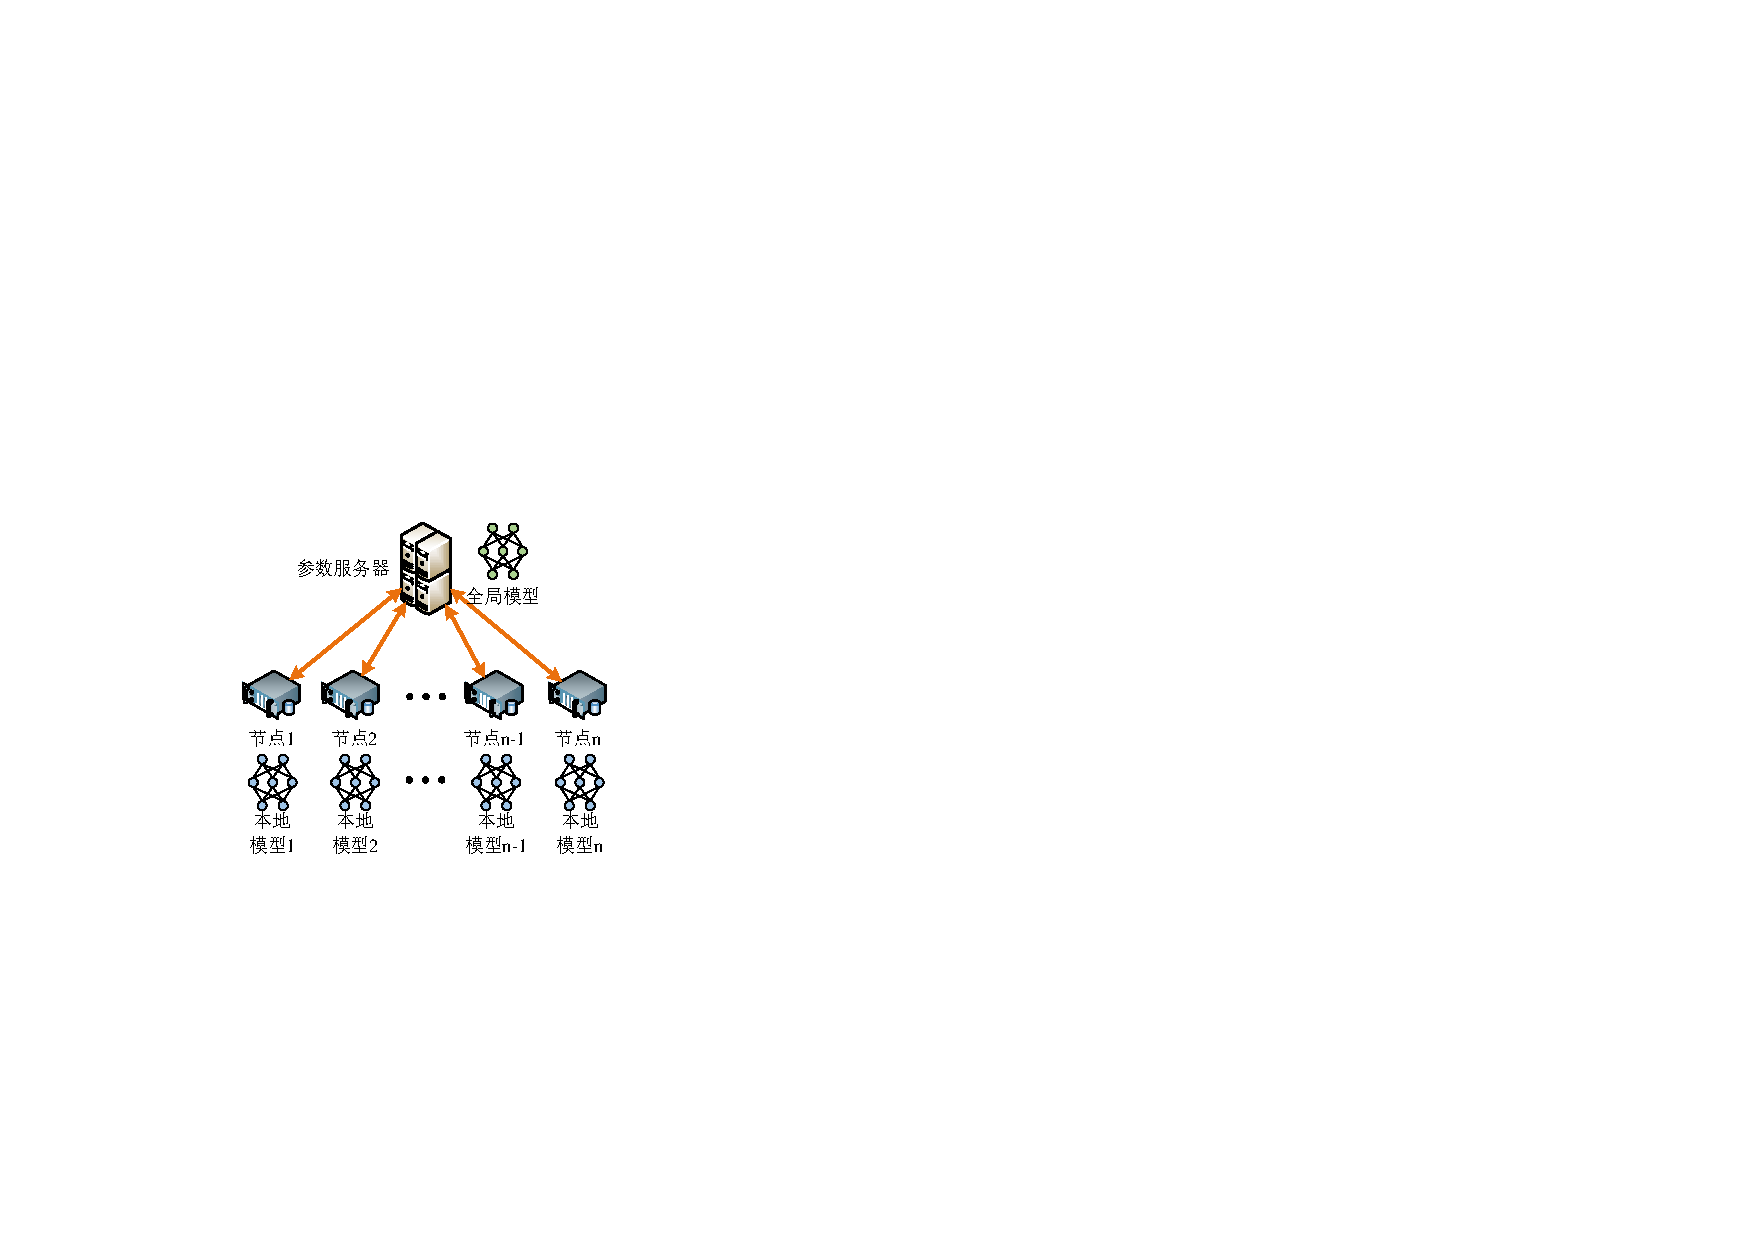
\includegraphics[width=0.3\linewidth]{figure/chapter1/fig1-3-PS.pdf}
%         \label{fig:Fig1-3-PS}
%     }
%     \subfigure[All-Reduce架构]{
%         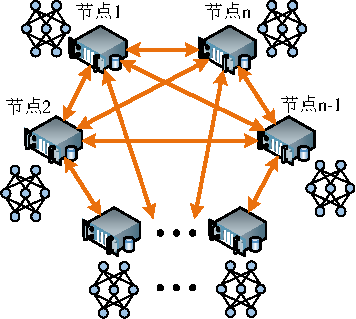
\includegraphics[width=0.3\linewidth]{figure/chapter1/fig1-3-2-AllReduce.pdf}
%         \label{fig:Fig1-3-allreduce}
%     }
%     \subfigure[Gossip架构]{
%         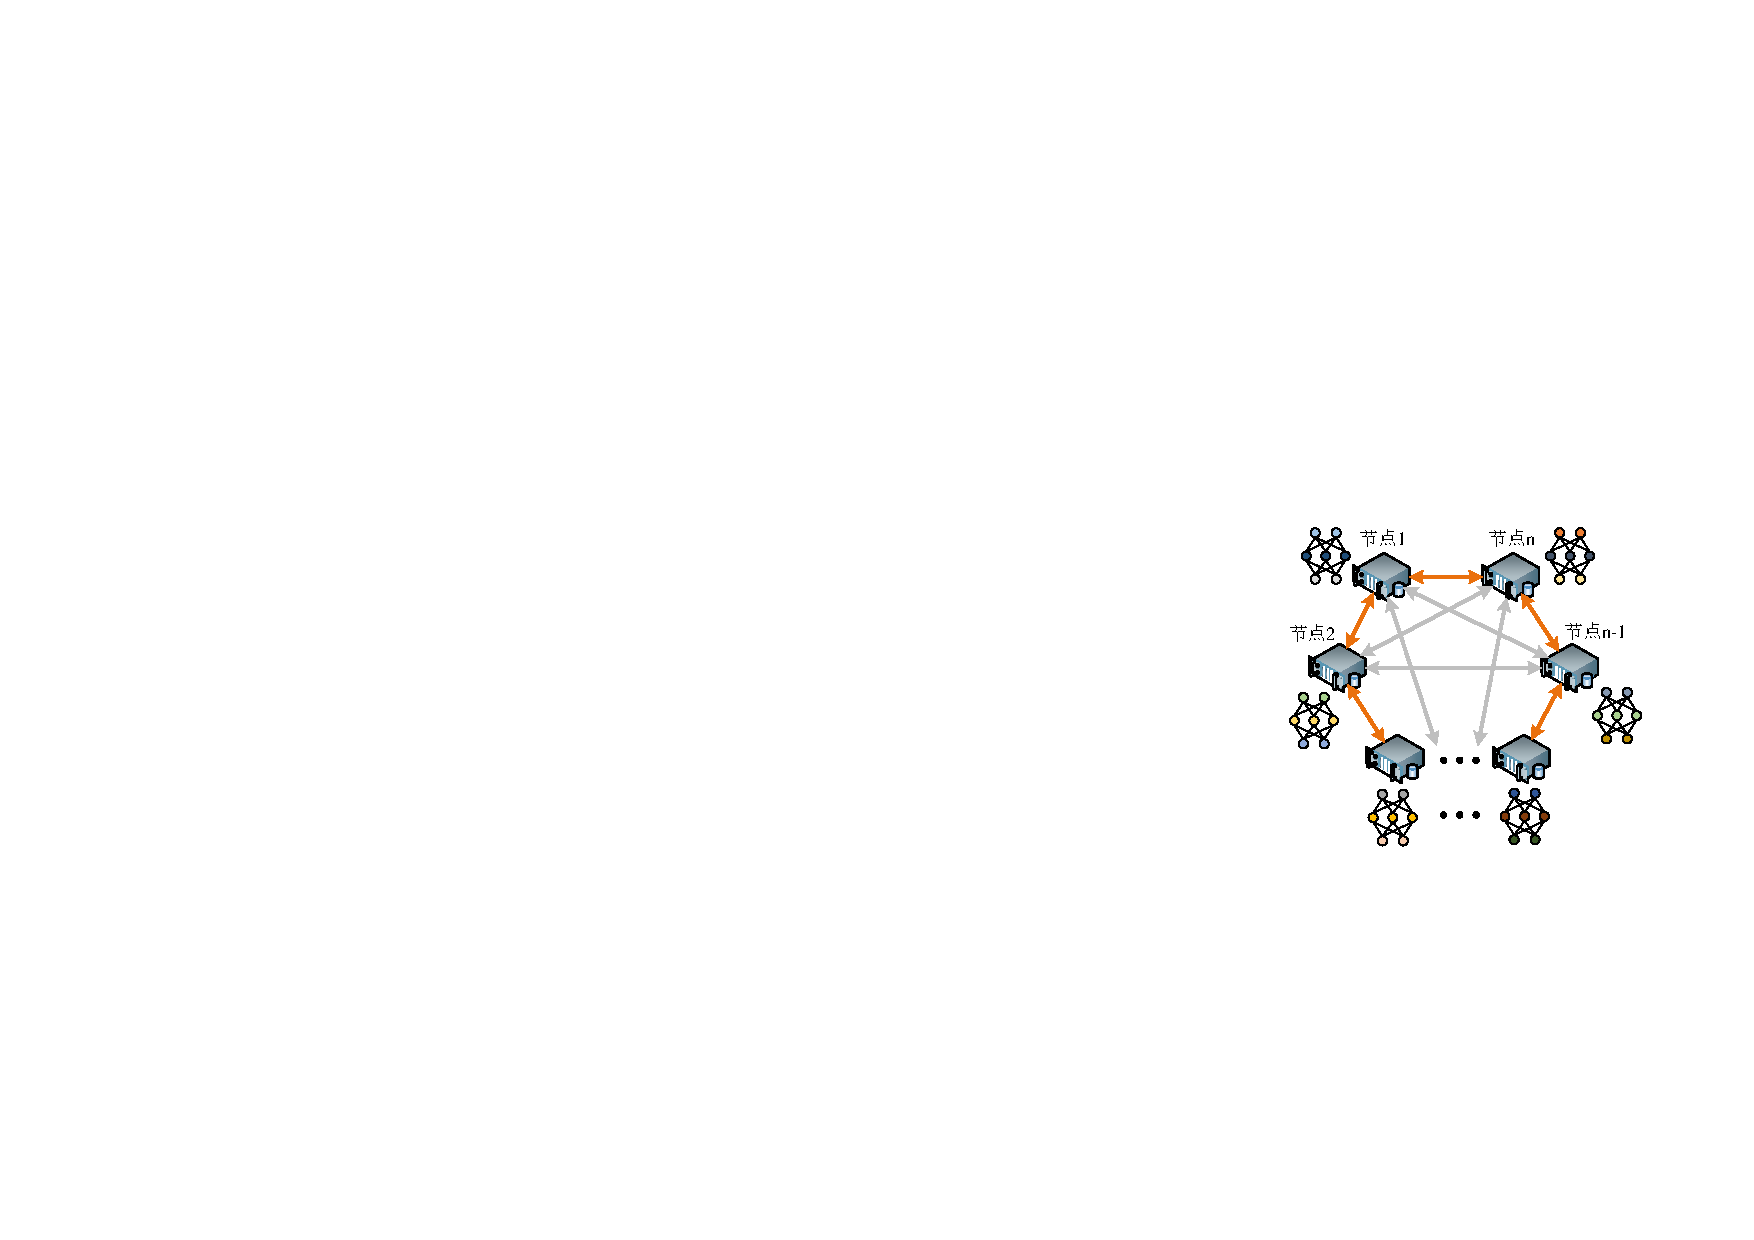
\includegraphics[width=0.3\linewidth]{figure/chapter1/fig1-3-3-Gossip.pdf}
%         \label{fig:Fig1-3-gossip}
%     }
%     \caption{分布式深度学习训练架构}
%     \label{fig:Fig1-3}
% \end{figure}

% 综上，随着模型规模与训练并行度的持续提升，通信效率逐步成为限制分布式训练可扩展性的核心因素之一。围绕集合通信的算法与系统优化，不仅直接决定单次迭代开销，也会影响整体吞吐、资源利用率与训练成本。

\subsection{基于通信优化的分布式训练加速的必要性}

分布式训练的理想状态是获得接近线性的加速比，即随着计算节点数量的增加，整体训练时间能够近似按比例缩短。然而在实际系统中，加速比往往呈现出先提升后趋缓、甚至下降的趋势：当节点规模较小时，新增算力能够有效提升训练吞吐；而当规模进一步扩大，通信与同步开销迅速累积，部分设备需要等待全局同步而处于空闲状态，导致整体资源利用率下降\cite{王帅2022}。因此，通信系统的效率在很大程度上决定了分布式训练在大规模场景下是否具备良好的扩展性与长期可持续性。

从工程实现角度看，大模型训练中的通信并非零散发生，而是贯穿于每一次迭代，甚至渗透到网络的多个计算层级之中。在数据并行训练中，梯度同步通常通过 AllReduce 完成；在张量并行场景下，为保证数值语义的一致性，矩阵计算过程往往需要与 ReduceScatter 和 AllGather 交替执行；而在 MoE 等专家并行结构中，大规模特征重分发使 AlltoAll 成为频繁触发且位于关键路径上的通信操作。随着训练模式从单一并行逐步演进为多维度混合并行，集合通信的种类与调用频率显著增加，其在端到端训练时间中的占比也随之持续上升。

另一方面，实际集群的互连结构也在持续演化：机内可能同时存在 NVLink/HCCS、PCIe 等链路，机间通过 RoCE/InfiniBand 等网络互连，多级交换机引入端口并发与转发模式等约束。传统固定模板（如单一 Ring/Tree）在复杂拓扑下往往难以同时兼顾低时延与高带宽利用率，且对多链路并行能力挖掘不足。通信效率不足不仅会拉长训练时长，还会造成昂贵算力资源的闲置与能耗浪费。

基于上述现状，围绕通信进行系统化优化具有明确意义：一方面，通过改进集合通信算法本身，减少通信轮数、提升链路利用率，可直接降低算子时延；另一方面，通过面向具体物理拓扑的算法合成，可以在复杂交换机网络与异构链路环境下自动构造高质量的路由与并发方案；此外，将通信与计算进行更深层次的并行化调度，能够把一部分通信开销从关键路径中“隐藏”掉，进一步提升端到端吞吐。本文即围绕上述三条路径展开研究。

\subsection{基于通信优化的分布式训练加速的研究挑战}

尽管集合通信与通算并行方向已有大量研究积累，但要在真实系统中稳定获得可观收益仍面临多方面挑战，主要体现在以下三个层面：

\begin{itemize}
    \item [（1）] \textbf{多链路与层级互连下的集合通信算法设计难。} 现代集群同时包含多种链路与交换结构，链路带宽/时延差异显著且常具备双向并行能力。如何在不增加实现复杂度与额外同步开销的前提下，减少通信轮数、提升有效带宽，并兼顾单机与多机场景的可扩展性，是集合通信算法落地的关键难点。
    \item [（2）] \textbf{面向复杂拓扑的算法合成难以兼顾建模精度与求解效率。} 以优化问题形式合成集合通信调度能够获得更高自由度，但真实拓扑往往包含多级交换机、端口并发约束以及不同转发模式等细节，建模过粗会导致合成方案不可用或性能欠佳，建模过细又会使求解开销失控。如何在可控时间内合成高质量调度，并支持 AllGather、AlltoAll 等多类算子，是算法合成方向的现实挑战。
    \item [（3）] \textbf{张量并行场景下的计算通信并行优化难。} 张量并行中集合通信操作往往位于前向/反向的关键路径，并与矩阵计算存在严格依赖；直接异步化可能破坏数值语义，盲目拆分又会引入额外开销。如何通过算子等价变换与细粒度拆分，把通信调度到可与计算重叠的时间窗口中，并以低侵入方式集成到主流深度学习框架，是通算并行优化能否真正发挥作用的决定因素。
\end{itemize}

因此，面向真实的大规模训练系统，从“集合通信算法设计—集合通信算法合成—计算通信并行”三个层面探索可落地、可扩展的通信优化方案，对提升分布式训练效率具有重要理论价值与工程意义。

\section{国内外研究现状}

围绕分布式训练中的通信瓶颈，学术界与工业界已经形成了较为系统的研究体系。从问题形态上看，相关工作大致可以归纳为三类：\textit{（1）集合通信算法设计}，聚焦于为 AllReduce/AllGather/AlltoAll 等算子构造更高效的通信流程；\textit{（2）集合通信算法合成}，强调在给定物理拓扑与资源约束下自动合成调度；\textit{（3）计算通信并行优化}，通过调度与算子拆分将通信开销从关键路径中尽可能隐藏。下面将按上述脉络对国内外研究进展进行梳理。

\subsection{集合通信算法设计}

在分布式训练中，集合通信算子是在本地计算之后实现全局同步的重要组件。AllReduce 负责对多节点数据进行规约并广播结果，常用于数据并行的梯度聚合；AllGather/ReduceScatter 是 AllReduce 的常见分解形式，在张量并行与分片通信中频繁出现；而 AlltoAll 则在混合专家等场景中承担跨节点特征重分发任务。围绕这些算子的高效实现，业界形成了 NCCL、HCCL 等高性能通信库，并在其中集成了多种经典算法。

按照通信策略是否显式感知物理拓扑，可将集合通信算法粗略分为两类：一类以固定逻辑拓扑为核心（如 Ring、Tree），算法流程相对稳定；另一类强调根据物理拓扑结构与链路特性构造调度，更关注多链路并发与层级互连的利用。

在固定逻辑拓扑算法中，Ring AllReduce 是最经典的实现之一。该算法在高性能计算领域被证明具有带宽最优性质\cite{patarasuk2009bandwidth}，并被引入深度学习训练实践\cite{gibiansky2017hpc}。Ring AllReduce 将节点组织成环形逻辑拓扑，整体流程可视为前 $(n-1)$ 轮 ReduceScatter 与后 $(n-1)$ 轮 AllGather 的串联：通过数据切分与逐轮转发，最终每个节点获得全量规约结果。其优势在于通信负载均衡、实现简洁；不足在于通信轮数随节点数线性增长，且在多链路并存环境下容易受制于最慢链路与固定调度模式。

为降低时延开销并适配更复杂的互连结构，研究者提出了多种分层与多维拓展。索尼提出的 2D-Torus\cite{mikami2018massively} 将设备排列为二维网格，通过分维度执行 ReduceScatter/Ring AllReduce/AllGather 来提升并行度；谷歌在 TPU 等专用互连硬件上对其流程进行了简化与优化\cite{ying2018image}。树形规约同样是一条重要路线，例如递归二分与倍增（HD）AllReduce\cite{thakur2005optimization}以 $\log_2 n$ 轮完成规约与分发，阿里巴巴在自建集群 EFLOPS 中采用该思路提升训练效率\cite{dong2020eflops}。在实际工程实现中，通信库常会结合多种拓扑模板：例如 NCCL 在不同版本中引入双二叉树等结构，以改善跨服务器场景的性能\cite{sanders2009two}。

随着集群规模扩大与链路层级增多，单一逻辑拓扑往往难以充分发挥硬件潜力，拓扑感知的算法设计逐渐成为热点。这类方法通常对系统互连结构进行分组或分层，在高带宽域内采用更激进的并发策略，在低带宽域内控制通信流量与同步次数。腾讯提出的分层 Ring AllReduce\cite{jia2018highly}即通过“组内—组间—组内”的层级流程，兼顾机内高带宽与机间低带宽差异。IBM 的 BlueConnect\cite{cho2019blueconnect}进一步将 AllReduce 分解为多阶段的 ReduceScatter/AllGather操作，并通过整数分解构造多维分组，以增强对多层网络的适配能力。针对分层通信的改进方向，还包括通过流水线并行掩盖部分通信开销等工作\cite{thao2021efficient}。

总体而言，集合通信算法设计已形成从固定模板到拓扑感知的多种范式，但在“多链路并行、双向全双工、层级互连”等新硬件特征下，仍存在通信轮数偏多、链路利用不足或调度不够灵活等问题。本文第2章将在环形算法框架内进一步挖掘双向链路并行能力，提出更低轮数、可工程落地的双半环集合通信算法。

\subsection{集合通信算法合成}

相比于人为设计通信模板，算法合成希望在给定物理拓扑与资源约束条件下，自动合成集合通信的路由与调度，从而避免固定框架下的性能上限，并提升对非对称与异构系统的适配性。该方向通常将合成问题建模为约束优化或搜索问题，再利用求解器或启发式算法合成调度序列。

早期代表性工作 SCCL\cite{cai2021synthesizing}将集合通信合成编码为 SMT 问题，在小规模拓扑（如 DGX-1）上合成带宽最优或时延最优的新算法，但模型规模与求解复杂度限制了其扩展性。随后，TACCL\cite{shah2023taccl}将问题转化为混合整数线性规划（MILP），并结合拓扑先验与分段求解降低复杂度，以适配更大规模场景。Themis\cite{rashidi2022themis}从多维异构网络角度出发，通过贪心分配数据块实现跨维度负载均衡，提升链路利用率并缩短算子时延。

在自动化与通用性方面，Won 等人提出 TACOS\cite{won2024tacos}，引入时间扩展网络（TEN）表示，将合成过程转化为“数据块—链路”匹配问题，并采用启发式贪心策略在约束下逐步满足后置条件。与此同时，TECCL\cite{liu2024rethinking}借鉴流量工程思想，对路由、容量与时序进行统一建模，并以 MILP 形式求解，在复杂拓扑上具备较强表达能力。除此之外，也有通过构建生成树或森林结构来合成集合通信算法的研究\cite{wang2020blink,zhao2024forestcoll}。

现有合成方法大体呈现两类取舍：一类依赖 SMT/MILP 等精确或近似求解器，调度质量较高但求解开销可能随拓扑规模急剧增长；另一类采用启发式策略或图搜索方法，易于扩展但需要在建模精度、算子类型与系统约束覆盖范围上做权衡。尤其在多级交换机拓扑中，端口并发、转发模式与链路占用会显著影响可行性与性能，现有方法要么建模不足、要么求解时间难以接受。针对这一现实需求，本文第3章将以 TEN 为基础，设计交换机拓扑感知的通用合成框架，在可控开销下合成高效 AllGather/AlltoAll 算法。

\subsection{计算通信并行优化}

除了优化通信算子本身，另一条重要思路是通过调度把通信开销“藏”到计算过程中，即提升计算与通信的重叠度。该方向的关键在于识别依赖关系与关键路径，并将可并行的通信提前发起或拆分为更细粒度的异步操作。

在数据并行场景中，经典方法通过按层拆分梯度并与反向传播重叠（如 WFBP\cite{zhang2017poseidon}），减少尾部等待。Zhang 等人提出 DeAR\cite{zhang2023dear}，将 AllReduce 拆分为 ReduceScatter 与 AllGather，并分别与反向与前向阶段并行，从而在更大程度上消除同步阻塞。

在流水并行场景中，研究重点转向对跨阶段依赖的调度优化。WPipe\cite{yang2022group}通过将激活值/梯度通信与前向、反向及重计算过程交错执行，提高重叠度并缓解气泡。MegaScale\cite{jiang2024megascale}系统分析 3D 并行中的依赖关系，对非关键路径操作进行隐藏；针对流水并行，其通过解耦发送/接收并异步启动实现更充分的重叠。Zero Bubble\cite{qi2024zero}进一步从算子拆分与异步参数更新角度降低理论气泡率。

张量并行与专家并行引入了更高频、更细粒度的集合通信，其通算并行优化更依赖算子层面的等价变换与融合。Collective Einsum\cite{wang2022overlap}通过分块矩阵计算与非阻塞通信实现细粒度并行；Oases\cite{li2023automated}针对启用重计算的张量并行训练给出自动化调度；CoCoNet\cite{jangda2022breaking}通过调整 ReduceScatter/AllGather 与算子执行顺序并进行融合，实现矩阵计算与通信并行。工业界也提出了面向特定算子的融合实现，如 Embedding 与 AlltoAll 的融合\cite{punniyamurthy2024optimizing}，以及将 GEMM 与通信并行并结合近内存计算的 T3\cite{pati2024t3}，Flux\cite{chang2024flux}则针对 ReduceScatter/AllGather 与 GEMM 的重叠进一步优化。

总体来看，通算并行优化已经从“数据并行按层重叠”发展到面向多并行策略的细粒度调度。然而，在张量并行场景中，通信与计算依赖更紧，且优化方案往往需要与深度学习框架、算子实现与通信库紧密配合，如何在低侵入、可复现的前提下稳定获得端到端收益仍值得深入研究。本文第4章将面向 Megatron 风格张量并行，提出基于算子拆分与调度的计算通信并行方法，并在 TP/DP 混合训练中进行验证。

\section{本文主要研究内容}
\subsection{研究思路与创新点}

结合前文背景与研究现状可以看到，分布式训练的通信优化正在从“单一算子模板优化”走向“面向真实拓扑的自动化调度”与“算子级通算协同”。围绕这一趋势，本文以集合通信为核心，面向多链路与多级交换机互连环境，开展三方面研究：首先，在存在双向并行环形链路的物理系统中，通过改造传统 Ring 流程减少通信轮数、提升有效带宽；其次，面向包含交换机节点与端口并发约束的真实拓扑，设计可扩展的集合通信算法合成框架，自动合成 AllGather/AlltoAll 算法；最后，针对张量并行训练中全局同步通信导致计算资源闲置的问题，提出基于算子拆分与调度的计算通信并行方法隐藏通信开销，以降低端到端训练时间。整体研究思路如\autoref{fig:framework}所示。

\begin{figure}[!htbp]
    \centering
    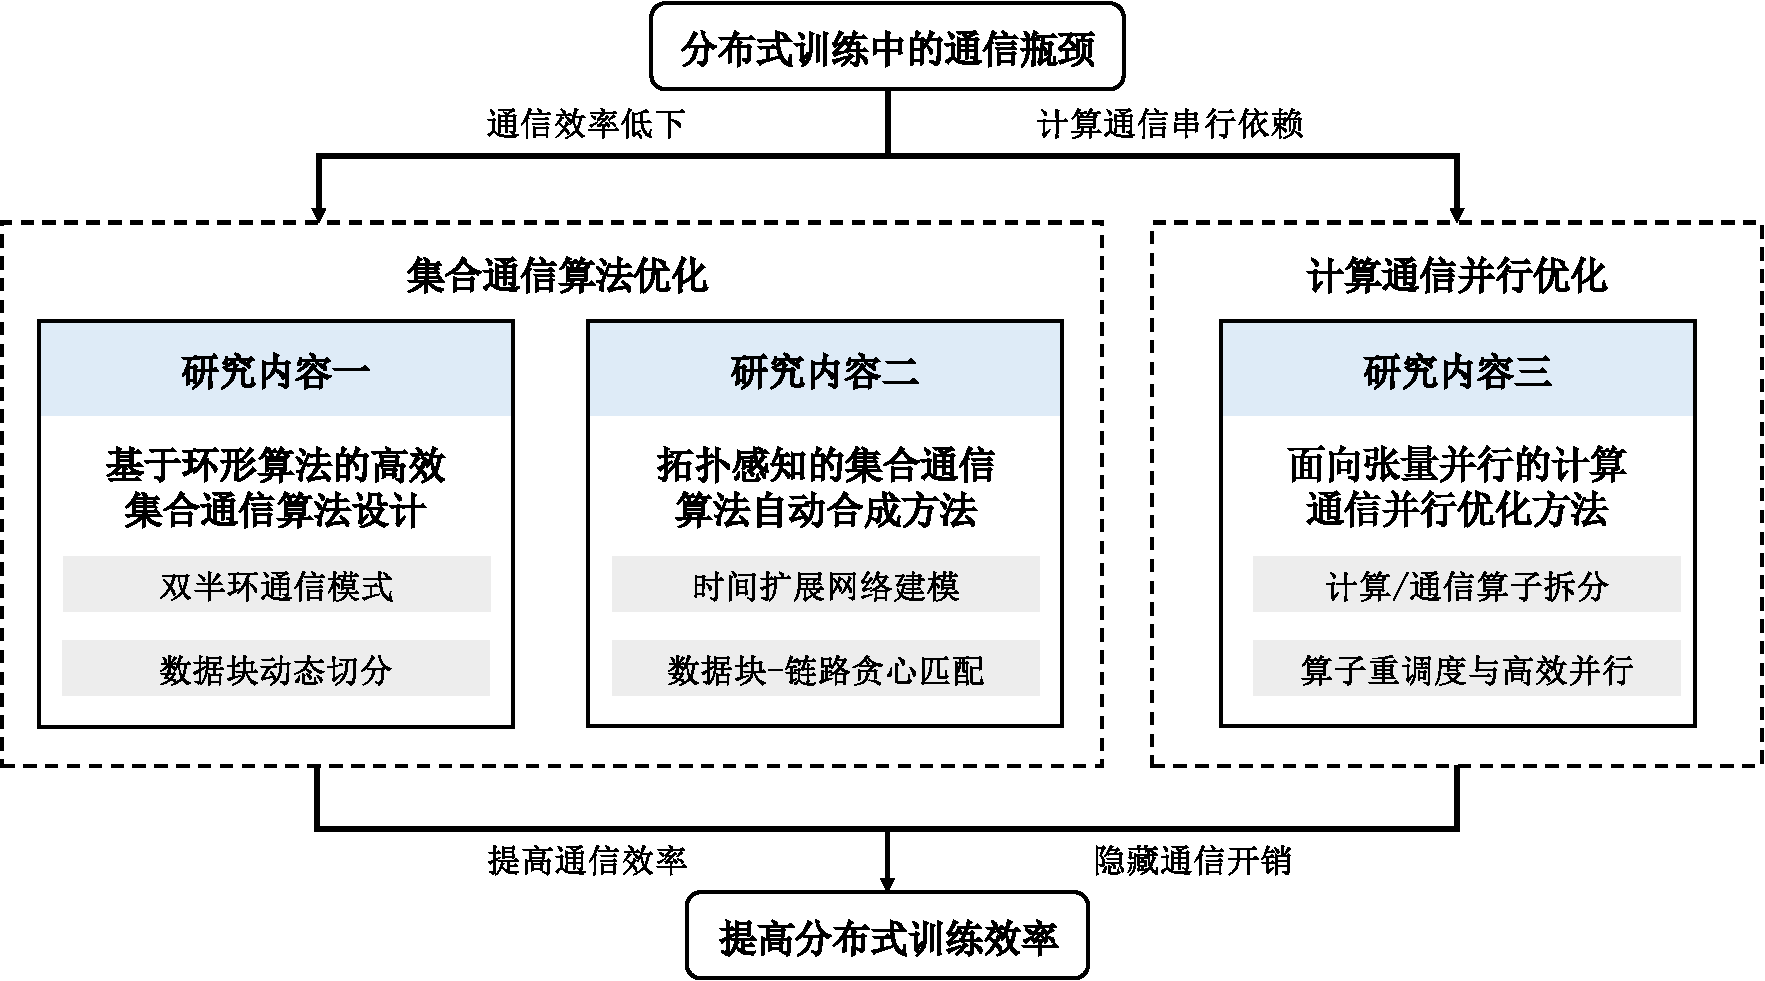
\includegraphics[width=\linewidth]{figure/chapter1/framework.pdf}
    \caption{\label{fig:framework}论文研究内容框架图}
\end{figure}

本文的主要创新点可概括为以下三点：
\begin{itemize}
  \item \textbf{提出链路聚合的双半环集合通信算法。} 针对双向全双工链路场景下传统双向 Ring 仍存在通信轮数偏多、有效带宽利用不足的问题，本文设计了双半环通信模式，使两组反向链路在更少轮次内完成数据扩散与规约，适用于 AllGather、ReduceScatter 与 AllReduce 等算子，并给出了多机场景下的分层扩展方式。基于 HCCL 的实现与实验表明，该算法在多种节点规模与数据量配置下均能稳定提升算法带宽，尤其在中等数据量场景中优势更为明显。
  \item \textbf{提出交换机拓扑感知的通用集合通信算法合成器FTACAS。} 针对现有合成方法对多级交换机拓扑支持不足或求解开销过高的问题，本文以物理拓扑为输入显式建模设备/交换机节点、链路时延与带宽、端口并发容量及转发模式，在 $\alpha$--$\beta$ 传输模型基础上构建时间扩展网络，并采用事件驱动的贪心合成框架合成调度。FTACAS 同时支持 AllGather 与 AlltoAll 两类基础算子，在多种典型拓扑上的评估显示其在保持较高算法带宽的同时显著降低合成时间开销，具备更好的工程可扩展性。
  \item \textbf{提出面向张量并行的计算通信并行优化方法。} 针对 Megatron 风格张量并行中同步通信阻塞严重的问题，本文通过将关键通信（如 AllReduce）进行等价拆分，并与矩阵计算单元进行细粒度重排与调度，在计算流与通信流之间建立并行执行机制。实验结果表明，在 TP/DP 混合并行训练中，该方法能够在不改变训练语义的前提下显著隐藏通信开销，降低端到端训练时间并提升整体吞吐。
\end{itemize}

\subsection{具体内容与章节安排}

本文各章节研究内容安排如下：

第一章，绪论。介绍分布式深度学习的发展背景，分析通信瓶颈对训练效率的影响，梳理集合通信算法设计、算法合成以及计算通信并行优化等方向的国内外研究现状，并概述本文的研究思路、创新点与章节结构。

第二章，基于环形算法的高效集合通信算法设计。介绍集合通信与环形算法基础，提出链路聚合的双半环算法，并给出其在 AllGather/ReduceScatter/AllReduce 三种算子下的实现方法，并进行了理论性能分析；最后在昇腾 910C 集群上实现并评估算法性能。

第三章，拓扑感知的集合通信算法合成方法。分析现有 TEN 合成方法的局限，提出交换机拓扑感知的通用合成器 FTACAS，给出拓扑建模、TEN 构建、事件驱动匹配策略以及针对 AllGather/AlltoAll 的关键设计，并在多种典型 GPU 拓扑上与 TECCL 等方法对比验证其合成效率与性能。

第四章，分布式训练中的计算通信并行优化方法。针对张量并行训练场景，分析 Transformer 与 Megatron 张量并行方法中的计算通信依赖关系，提出基于算子拆分调度的通算并行方案，并在 TP/DP 混合训练任务上进行实验验证与 Profiling 分析。

第五章，总结与展望。总结全文工作与创新点，并对后续研究方向进行展望。
